
\section*{Differentiation}
\subsubsection*{Uden hjælpemidler}
\subsection*{Niveau 1}
Bestem den afledede funktion til følgende funktioner:
\begin{align*}
	&1) \ 2x^2 + 10x^3 &&2) \ 5\sqrt{x} \\
	&3) \ \cos(x)-10 &&4) \ \ln(x)-\sqrt{7} \\
	&5) \ \textnormal{e}^{7}+\ln(4) &&6) \ -5x^{\frac{3}{2}} \\
\end{align*}

\subsection*{Niveau 2}
Bestem den afledte funktion til følgende funktioner:
\begin{align*}
	&1) \ \ln(x^2+11x-6) &&2) \ \cos(x)\cdot(4x^2-3x^5) \\
	&3) \  8\sqrt{x}\cdot \textnormal{e}^{x} &&4) \ \textnormal{e}^{4\sin(x)}\\
	&5) \ 2^{5x+11} &&6) \ \frac{x^{\frac{1}{2}}}{-2\ln(x)} \\
\end{align*}

\subsection*{Niveau 3}
Bestem den afledte funktion til følgende funktioner:
\begin{align*}
	&1) \ \cos(x^2)\cdot \sin(4x+13) &&2) \ \textnormal{e}^{\sqrt{x}\cdot \sin(x)} \\
	&3) \ \sqrt{x^4-2x^2}\cdot \ln(x^2-2x^2) &&4) \ (\cos(x)\cdot \sin(x))^{\frac{\cos(x)}{\sin(x)}}
\end{align*}

\newpage

\section*{Væksthastighed og tangenthældning}
\subsubsection*{Uden hjælpemidler}
\subsection*{Niveau 1}

\begin{enumerate}[label=\roman*)]
	\item En funktion $f$ er givet ved
	\begin{align*}
		f(t) = 6t^2-11t+7.
	\end{align*}
	Bestem væksthastigheden for $f$ til tidspunktet $t = 4$.
	\item En funktion $g$ er givet ved
	\begin{align*}
		g(x) = \ln(x)+4x.
	\end{align*}
	Bestem tangenthældningen for grafen for $g$ i punktet $(1,g(1))$.
	\item En funktion $h$ er givet ved
	\begin{align*}
		h(x) = x^2-4x+11.
	\end{align*}
	Bestem det sted, hvor tangenthældningen for grafen for $h$ er 2.
	
\end{enumerate}

\subsection*{Niveau 2}

\begin{enumerate}[label=\roman*)]
	\item En funktion $f$ er givet ved
	\begin{align*}
		f(t) = t^3 - 3t^2 + 4.
	\end{align*}
	Bestem de steder, hvor vækshastigheden er nul.
	\item En funktion $g$ er givet ved
	\begin{align*}
		g(x) = \ln(x)+2\sqrt{x}+4
	\end{align*}
	Bestem ligningen for tangenten til grafen for $g$ gennem punktet $(1,g(1))$. 
	\item En funktion $h$ er givet ved
	\begin{align*}
		h(x) = \cos(x)\cdot(6x^2+4x+7).
	\end{align*}
	Bestem $h'(0)$.

\end{enumerate}

\subsection*{Niveau 3}

\begin{enumerate}[label=\roman*)]
	\item En funktion $f$ er givet ved
	\begin{align*}
		f(x) = x^3 + 3x^2 - 4x + k.
	\end{align*}
	Bestem de værdier for $k$, så $f$ har linjen med ligningen $y = 16x-10$ som tangent
	\item En funktion $h$ er givet ved
	\begin{align*}
		h(x) = x^3-3x^2+3x+4.
	\end{align*}
	Bestem tallet $a$, så ligningen $h'(x) = a$ har så få løsninger som muligt.
\end{enumerate}

\subsubsection*{Med hjælpemidler}

\subsection*{Niveau 1}
I en begrænset tidsperiode kan antallet af bakterier i en petriskål beskrives ved
\begin{align*}
	B(t) = 17.32\textnormal{e}^{0.017t},
\end{align*}
hvor $t$ beskriver tiden i timer efter begyndelsestidspunktet og $B$ er antallet af bakterier i mia. 

\begin{enumerate}[label=\roman*)]
	\item Tegn grafen for $B$
	\item Bestem $B(3)$ og $B'(3)$ og forklar hvad disse tal siger om bakterievæksten.
	\item Hvornår stiger antallet af bakterier med én mia. i timen?
\end{enumerate}

\subsection*{Niveau 2}

Antallet af mennesker i en storby $P$ kan i tidsperioden 1930 til 2020 beskrives ved funktionen
\begin{align*}
	P(t) = \frac{7.8}{1+5.6\textnormal{e}^{-0.074t}},
\end{align*}
hvor $P$ er antal mennesker i mio. og $t$ er tiden efter år 1930 i år. 
\begin{enumerate}[label=\roman*)]
	\item Tegn funktionen.
	\item Bestem $P(0)$ og giv en fortolkning af dette tal.
	\item Bestem $P'(40)$ og forklar, hvad dette tal siger om udviklingen. 
	\item Bestem det tidspunkt, hvor antallet af mennesker i byen vokser mest. 
\end{enumerate}

\subsection*{Niveau 3}
Antallet af katte i et lille land kan beskrives ved funktionen 
\begin{align*}
	K(t) = \frac{5.3}{1+c\textnormal{e}^{-0.097t}},
\end{align*}
hvor $K$ er antallet af katte i mio. og $t$ er tiden i år efter år 1950.

\begin{enumerate}[label=\roman*)]
	\item Bestem antallet af katte i år 1960, hvis $c = 4.4$.
	\item Hvornår stiger antallet af katte med $100000$ årligt, hvis $c = 4.9$?
	\item Hvor mange katte er der i år 1960, hvis antallet af katte skal vokse hurtigst i år 1980?
\end{enumerate}

\newpage
\section*{Grafer og differentialregning}

\subsubsection*{Uden hjælpemidler}

Bestem hvilke af graferne der tilsvarer funktionen $f$ og hvilken der tilsvarer $f'$
\begin{center}

\scalebox{0.6}{
	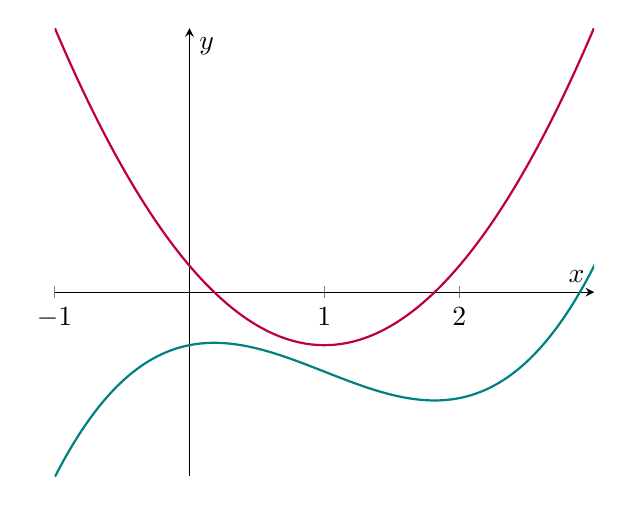
\begin{tikzpicture}
		\begin{axis}[axis lines = middle, xmin = -1, xmax = 3, xtick = {-1,1,2}, ytick = {0},
		xlabel = $x$, 
		ylabel = $y$]
			\addplot[samples = 1000, color = teal, thick] {x^3-3*x^2+x-2};
			\addplot[samples = 1000, color = purple, thick] {3*x^2-6*x+1};
		\end{axis}
	\end{tikzpicture}
	}
	\qquad
\scalebox{0.6}{
	\begin{tikzpicture}
		\begin{axis}[axis lines = middle, xmin = 0.1, xmax = 2, xtick = {1}, ytick = {0},
		xlabel = $x$, 
		ylabel = $y$]
			\addplot[samples = 1000, color = teal, thick] {1/x - 2*x};
			\addplot[samples = 1000, color = purple, thick] {ln(x)-x^2};
		\end{axis}
	\end{tikzpicture}
}

\scalebox{0.6}{
	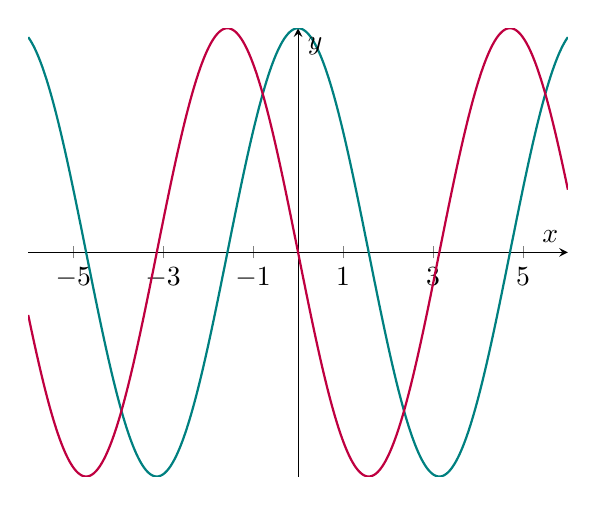
\begin{tikzpicture}
		\begin{axis}[axis lines = middle, xmin = -6, xmax = 6, xtick = {-5,-3,-1,1,3,5}, ytick = {0},
		xlabel = $x$, 
		ylabel = $y$]
			\addplot[samples = 1000, color = teal, thick, domain = -6:6] {cos(deg(x))};
			\addplot[samples = 1000, color = purple, thick, domain = -6:6] {-sin(deg(x))};
		\end{axis}
	\end{tikzpicture}
	}
	\qquad
\scalebox{0.6}{
	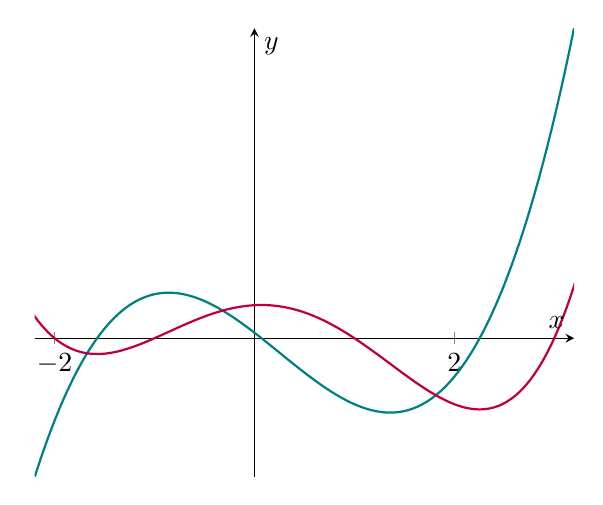
\begin{tikzpicture}
		\begin{axis}[axis lines = middle, xmin = -2.2, xmax = 3.2, xtick = {-2,2}, ytick = {0},
		xlabel = $x$, 
		ylabel = $y$]
			\addplot[samples = 1000, color = teal, thick] {4*x^3-3*x^2-14*x+1};
			\addplot[samples = 1000, color = purple, thick] {(x-1)*(x-3)*(x+1)*(x+2)};
		\end{axis}
	\end{tikzpicture}
}
\end{center}

\newpage
\section*{Monotoniforhold}

\subsubsection*{Uden hjælpemidler}
\begin{enumerate}[label=\roman*)]
	\item For en funktion $g$ gælder der, at $g'(x) = 0$ hvis og kun hvis $x = 2$ eller $x = 4$ samt at $g'(-4) = 1$, $g'(3) = 2$ og $g'(5) = -2$.   
	Opskriv monotoniforholdene for $g$	
	\item Bestem monotoniforholdene for funktionen $f$ givet ved
	\begin{align*}
		f(x) = x^2 -x - 2
	\end{align*}
	\item Bestem monotoniforholdene for funktionen $g$ givet ved
	\begin{align*}
		x^3 - 3x^2 + 3x + 10
	\end{align*}

\end{enumerate}
\newpage


\section*{Optimering }
\subsubsection*{Med hjælpemidler}

\subsubsection*{Niveau 2}
En person skal indhegne sine høns, og han vælger at gøre det op ad en bygning. Han skal derfor have hegn på det stiplede område på figuren. 
\begin{enumerate}[label=\roman*)]
	\item Bestem et udtryk for omkredsen af hegnet, der afhænger af $b$ og $l$.
	\item Bestem et udtryk for arealet af hegnet, der afhænger af $b$ og $l$. 
	\item Udnyt at personen har 50m hegn til at bestemme et udtryk for arealet, der kun afhænger af bredden.
	\item Bestem de dimensioner, der gør hønseburet så stort som muligt. 
\end{enumerate}
\begin{center}
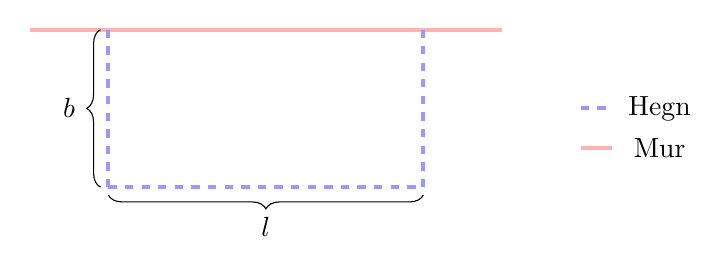
\begin{tikzpicture}
\draw[line width = 0.5mm,color=red!30] (-3,0) -- (3,0);
\draw[line width = 0.5mm, dashed, color = blue!40] (-2,0) -- (-2,-2);
\draw[line width = 0.5mm, dashed, color = blue!40] (-2,-2) -- (2,-2);
\draw[line width = 0.5mm, dashed, color = blue!40] (2,-2) -- (2,0);
\draw[line width = 0.5mm, dashed, color = blue!40] (4,-1) -- (4.4,-1);
\draw[line width = 0.5mm, color=red!30] (4,-1.5) -- (4.4,-1.5);
\node at (5,-1) {Hegn};
\node at (5,-1.5) {Mur};
\draw [decorate,decoration = {brace,mirror,amplitude = 5pt}] (-2.1,-0.0) --  (-2.1,-2);
\draw [decorate,decoration = {brace,mirror,amplitude = 5pt}] (-2,-2.1) --  (2,-2.1);
\node at (-2.5,-1) {$b$};
\node at (0,-2.5) {$l$};
\end{tikzpicture}
\end{center}
\subsubsection*{Niveau 3}
Vi skal bygge en pyramide, og vi har sten nok til at overfladearealet af pyramiden kan blive 1 km$^2$. Vi vil gerne have at pyramiden har kvadratisk bund, og vi ønsker, at rumfanget af pyramiden er så stort som muligt, og vi ønsker ikke, at der skal være bund i pyramiden. Bredden og længden af pyramiden er $x$ og højden af pyramiden er $h$. Pyramiden kan ses på Fig. \ref{fig:pyramide2}
\begin{figure}[H]
\centering
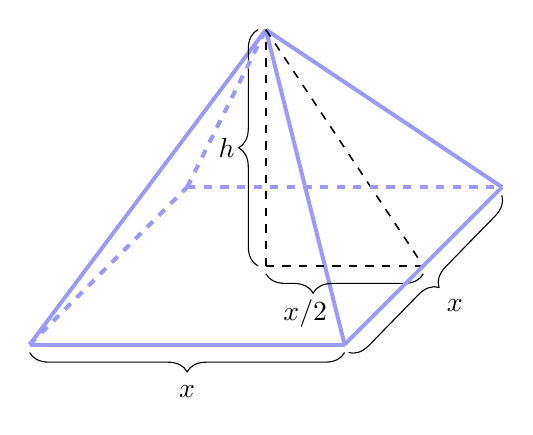
\begin{tikzpicture}
\draw[line width = 0.5mm,  color = blue!40] (0,0) -- (4,0);
\draw[line width = 0.5mm,  color = blue!40] (0,0) -- (3,4);
\draw[line width = 0.5mm,  color = blue!40] (4,0) -- (3,4);
\draw[line width = 0.5mm,  color = blue!40] (6,2) -- (3,4);

\draw[line width = 0.2mm, dashed] (3,1) -- (3,4);
\draw[line width = 0.2mm, dashed] (3,1) -- (5,1);
\draw[line width = 0.2mm, dashed] (3,4) -- (5,1);

\draw[decorate,decoration = {brace,amplitude = 7pt}] (3-0.1,1) -- (3-0.1,4);
\draw[decorate,decoration = {brace,mirror,amplitude = 7pt,aspect = 0.3}] (3,1-0.1) -- (5,1-0.1);

\draw[line width = 0.5mm,  color = blue!40] (4,0) -- (6,2);

\draw[line width = 0.5mm, dashed,  color = blue!40] (0,0) -- (2,2);
\draw[line width = 0.5mm, dashed,  color = blue!40] (2,2) -- (6,2);
\draw[line width = 0.5mm, dashed,  color = blue!40] (2,2) -- (3,4);



\draw [decorate,decoration = {brace,mirror,amplitude = 7pt}] (0,-0.1) --  (4,-0.1);
\draw [decorate,decoration = {brace,mirror,amplitude = 7pt}] (4.05,-0.1) --  (6,1.9);


\node at (2,-0.6) {$x$};
\node at (5.4,0.5) {$x$};
\node at (2.5,2.5) {$h$};
\node at (3.5,0.4) {$x/2$};
\end{tikzpicture}
\caption{Pyramide med kvadratisk bund}
\label{fig:pyramide2}
\end{figure}
\begin{enumerate}[label=\roman*)]
\item Rumfanget af en pyramide er givet ved $R = (b\cdot l\cdot h)/3$, hvor $l$ er længden af pyramiden, $b$ er bredden af pyramiden og $h$ er højden af pyramiden. Bestem overfladearealet af pyramiden på Figur \ref{fig:pyramide2}.
\item Argumentér for, at overfladeareal af en af de fire sidetrekanter er givet ved 
\begin{align*}
O_T = \frac{x\cdot\sqrt{\frac{x^2}{4}+h^2}}{2},
\end{align*}
og konkludér, at det samlede overfladeareal af pyramiden må være givet ved 
\begin{align*}
O_P = 2\cdot x\cdot \sqrt{\frac{x^2}{4}+h^2}.
\end{align*}

\item Udnyt, at vi ved, at det samlede overfladeareal skal være $1$km$^2$, således at 
\begin{align*}
O_P = 1 = 2\cdot x\cdot \sqrt{\frac{x^2}{4}+h^2},
\end{align*}
og brug dette til at vise, at 
\begin{align*}
h=\sqrt{\frac{1}{4\cdot x^2}-\frac{x^2}{4}}.
\end{align*}

\item Indsæt nu udtrykket for $h$ i udtrykket for rumfanget af pyramiden og plot rumfanget som funktion af $x$ på intervallet $[0,1]$. 
\item Bestem de dimensioner på pyramiden, der gør rumfanget af pyramiden maksimalt.
\end{enumerate}

